\section{Вычислительные эксперименты}
    Возьмём параметры для модели:
    \[
        \begin{split}
            & \xi_1 = 10, \xi_2 = 8, \xi_3 = 6, \\
            & \alpha_{12} = 6, \alpha_{13} = 2, \alpha_{23} = 0.5, \\
            & k_{12} = 4, k_{13} = 1, k_{23} = 0.5.
        \end{split}
    \]

    \subsection{При вымирании первой популяции}

    \begin{figure}[H]
        
        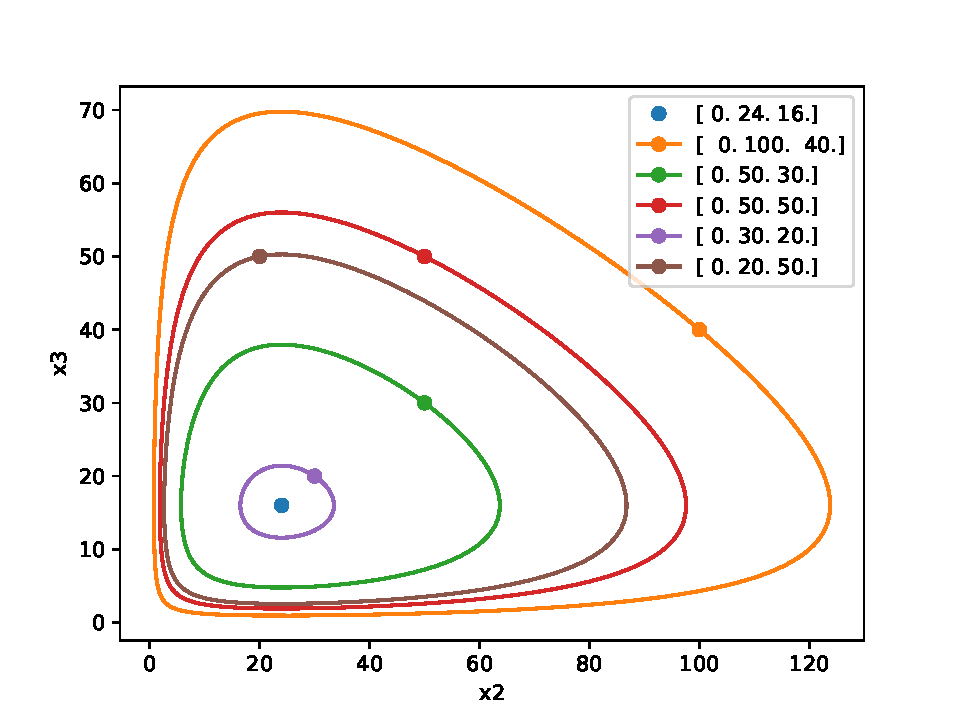
\includegraphics[width=8cm]{pictures/x1_0phase.pdf}
        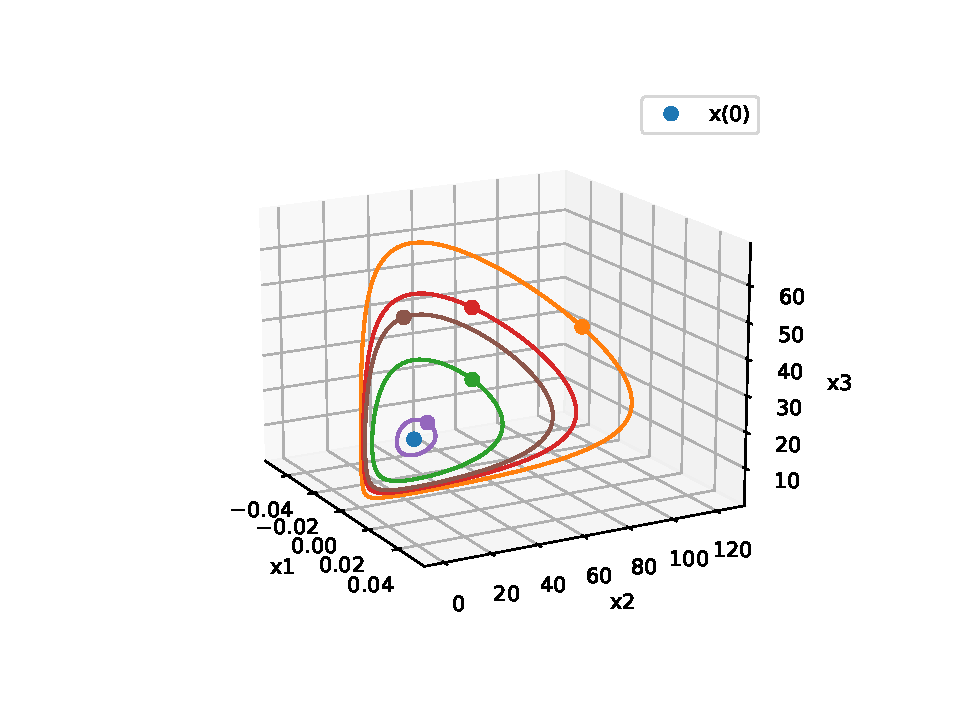
\includegraphics[width=8cm]{pictures/x1_0phase3.pdf}
        \caption{На отрезке времени \( [0, 3] \).}
    \end{figure}